\section{Subm\'odulo AD}

El subm\'odulo conversor anal\'ogico digital AD tiene 2 canales de adquisici\'on en paralelo
con una resoluci\'on de 12 bits por canal, una frecuencia de muestreo m\'axima de 10 Mhz 
y capacidad de almacenamiento en bloques de 1KB, 2KB, 4KB, 8KB, 16KB, 32KB, 64KB, 128KB.

\begin{table}[ht]
    \centering
    \begin{tabular}{|l|l|l|}
    \hline
     Direcci\'on   & Descripci\'on   & modo\\
    \hline
     0x0B        & comando y control & lectura/escritura\\ 
    \hline
     0x0C        & muestreo          & escritura\\
     \hline
     0x08        & canal B           &lectura   \\
     \hline
     0x09        & canal AB          &lectura   \\
     \hline
     0x0A        & canal A           &lectura   \\
     \hline
\end{tabular}
\caption{\label{tab:registros_ad} Registros del AD}
\end{table}

\subsection{Registro de comando}
\begin{table}[ht]
    \centering
    \begin{tabular}{|l|l|l|}
    \hline
    Bit    & Descripci\'on \\
    \hline
     0 & modo\\ 
    \hline
     1 & modo\\
     \hline
     2 & - \\
     \hline
     3 & - \\
     \hline
     4 & bloque \\
     \hline
     5 & bloque \\
     \hline
     6 & bloque \\
     \hline
     7 & reset \\
     \hline
\end{tabular}
\caption{\label{tab:registros_ad_cmd}Registro de comando.}
\end{table}

\subsection{Registro de datos}

\begin{table}[ht]
    \centering
    \begin{tabular}{|l|l|l|}
    \hline
    Direcci\'on & Descripci\'on \\
    \hline
     0x08 & canal B\\ 
    \hline
     0x09 & canal AB\\
     \hline
     0x0A & canal A\\
     \hline
\end{tabular}
\caption{\label{tab:registros_ad_datos}Registros de datos.}
\end{table}


\subsection{Configuraci\'on de un ciclo de adquisici\'on}

Un ciclo de adquisici\'on requiere la configuraci\'on del intervalo de muestreo
de acuerdo a la siguiente f\'ormula:
\begin{gather}
period = 100 ns\\
interval \in \mathbb{N} \land 0 < interval < 25500\\
n = interval / period\\
delta  = 255 - n\\
\end{gather}

\subsubsection{Configuraci\'on bloque de 1KB y muestreo 1 microsegundo}

\begin{algorithm}
    \caption{Configuraci\'on 1KB 1 microsegundo}\label{algo_ad_conf}
    \begin{algorithmic}[1]
    \Procedure{Setup()}{}
    \State
    \State $config \gets 0x00$
    \State $config \gets config \lor 0x02$
    \State $config \gets config \lor 0x80$
    \State $config \gets config \land 0xFE$
    \State $write(0x0B, config)$
    \State
    \State $config \gets 0x00$
    \State $config \gets config \lor 0x02$
    \State $config \gets config \land 0x7F$
    \State $config \gets config \lor 0x01$
    \State $write(0x0B, config)$
    \State
    \State $period \gets 100$
    \State $samples= 1000 / period$
    \State $delta = 255 - samples$
    \State $write(0x0C, delta)$

    \EndProcedure
    \end{algorithmic}
    \end{algorithm}
    \newpage
\subsection{Extracci\'on de los datos de la memoria interna}

El bus de datos de la memoria del AD es de 8 bits y las muestras de 12 bits,
siendo necesarias 3 lecturas de 8 bits y una operaci\'on de partici\'on para
obtener la muestra final de los canales A y B.

\begin{figure}[!htb].
    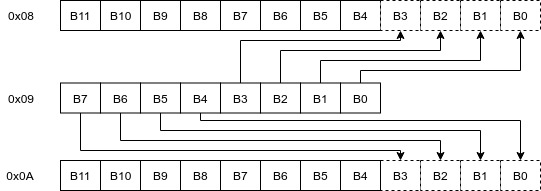
\includegraphics[width=\linewidth]{../figures/d8.jpg}
    \caption{Buffers del subm\'odulo AD}
    \label{fig:d8}
\end{figure}

Para la extracci\'on de los datos es necesaria esta serie de pasos:

\begin{itemize}
    \item modo PC, deshabilitada la adquisici\'on y reset contador de direcciones
    \item modo PC, deshabilitada la adquisici\'on y contador de direcciones en modo normal
    \item lectura del registro 0x08 del canal B
    \item modo PC, deshabilitada la adquisici\'on y reset contador de direcciones
    \item modo PC, deshabilitada la adquisici\'on y contador de direcciones en modo normal
    \item lectura del registro 0x0A del canal A
    \item modo PC, deshabilitada la adquisici\'on y reset contador de direcciones
    \item modo PC, deshabilitada la adquisici\'on y contador de direcciones en modo normal
    \item lectura del registro 0x09 con nibbles del canal A y B.
    \item armado de los datos de los respectivos canales.
\end{itemize}

\begin{algorithm}
    \caption{Extracci\'on de datos del AD}\label{algo_ad_data}
    \begin{algorithmic}[1]
    \Procedure{GetDataFromAD()}{}
   
    \State $config \gets 0x00$
    \State $config \gets config \lor 0x02$
    \State $config \gets config \lor 0x80$
    \State $config \gets config \land 0xFE$
    \State $write(0x0B, config)$
    \State $config \gets 0x00$
    \State $config \gets config \lor 0x02$
    \State $config \gets config \land 0x7F$
    \State $config \gets config \land 0xFE$
    \State $write(0x0B, config)$
    \State $A \gets read(0x08)$
    \State
    \State $config \gets 0x00$
    \State $config \gets config \lor 0x02$
    \State $config \gets config \lor 0x80$
    \State $config \gets config \land 0xFE$
    \State $write(0x0B, config)$
    \State $config \gets 0x00$
    \State $config \gets config \lor 0x02$
    \State $config \gets config \land 0x7F$
    \State $config \gets config \land 0xFE$
    \State $write(0x0B, config)$
    \State $B \gets read(0x0A)$
    \State
    \State $config \gets 0x00$
    \State $config \gets config \lor 0x02$
    \State $config \gets config \lor 0x80$
    \State $config \gets config \land 0xFE$
    \State $write(0x0B, config)$
    \State $config \gets 0x00$
    \State $config \gets config \lor 0x02$
    \State $config \gets config \land 0x7F$
    \State $config \gets config \land 0xFE$
    \State $write(0x0B, config)$
    \State $AB \gets read(0x09)$
    \State
    \State $sample\_A \gets join\_buffers(A, AB)$
    \State $sample\_B \gets join\_buffers(B, AB)$

    \EndProcedure
    \end{algorithmic}
    \end{algorithm}



\newpage
